\section{FTA}
A hibafa analízis az egyik legalaposabb és legáltalánosabb vizsgálati módszer.
Ha van olyan hibakövetkezmény, amit már az előzőleg végrehajtott módszerek felfedeztek, de bonyulultsága nem tette lehetővé, hogy részletesebben elemezzék akkor azt általában az FTA vizsgálja ki.

A dolgozatban ez a komplex alegység, melynek vizsgálatát erre a fejezetrészre hagytam, a vezérlő elektronika.
Ez az egység csak részben lett megemlítve az előző analízisek során és eddig a pontig csak annyit tudunk róla, hogy a WSP funkció, ami a mikroprocesszoron fut SIL2-es besorolást kapott.

\subsection{Kvalitatív analízis}
Ebben a részben azt a hibát kutatjuk - egyenlőre kvalitatív jellegel -, hogy mekkora valószínűséggel lesz detektálatlan hibamódban a vezérlő elektronika.

A részegység rendelkezik redundáns CAN kommunikációs interfésszel, amelyen képes adatokat fogadni és hibát is jelezni.
Az egész alaplap rendelkezik egy táppal, ami a vonat rendszerfeszültségéből képes a többi részegység által szükséges 5V feszültséget konvertálni.

Az alrendszer rendelkezik egy dedikált kommunikációs lehetőséggel, melyen a súlyos hibákat tudja jelezni a vonat szint (Train Level) felé. 
Elsődlegesen ez a hibajelző rendszer.

Továbbá, a vezérlési funkcióknak helyet adó mikroprocesszor található még az egységben.
Ez rendelkezik egy saját dedikált táppal, ami a $\mu C$-nek transzformálja a megfelelő feszültségszintet és a programkód számára elérhető memória modullal.

Ez alapján konstruálható olyan hibafa, ami a fent leírtak alapján helyezi el a hibamódokat.
Az elkészített hibafa a \ref{fig:qualit}. ábrán látható. Ezen látható, hogy nincsen teljesen normál formára hozva, hiszen a felső VAGY kapu alatt található még egy VAGY kapcsolat.
Ha teljesen normálalakúra alakítjuk az \emph{uC-FAILURE} kapu alatt lévő elemek egyenesen a Top-event alá kerülnek.
Így rendszerben hat darab minimális vágás található.

\begin{figure}
    \footnotesize
    \centering
    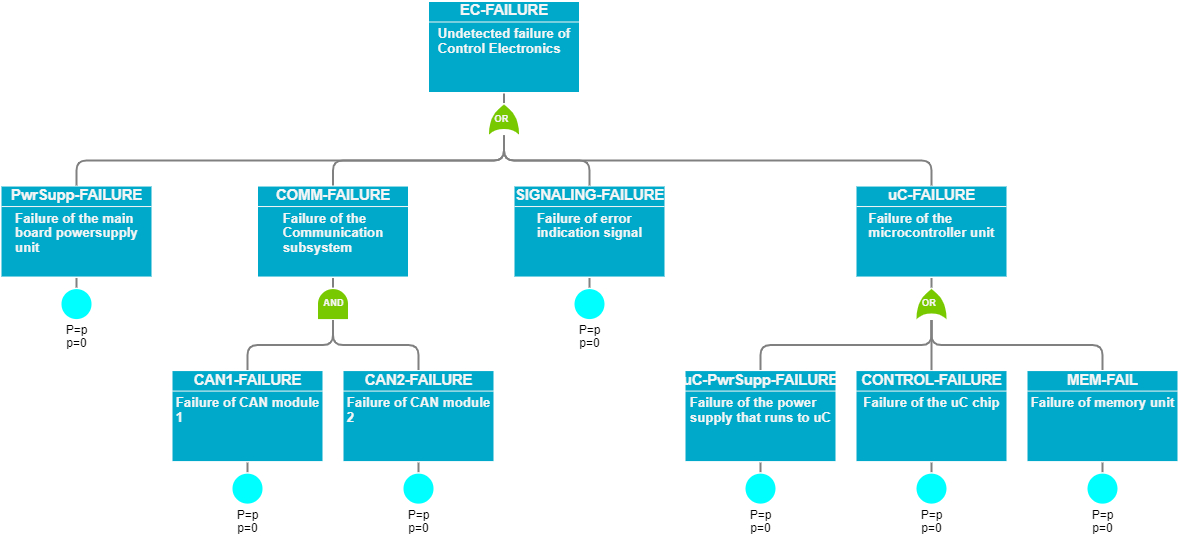
\includegraphics[width=150mm, keepaspectratio]{figures/QualitativeFTA.png}
    \caption{A vezérlőelektronika qualitatív hibafája.}
    \label{fig:qualit}
\end{figure}

\subsection{FIT allokáció}
A hibafa diagramm rendkívül alkalmas az alegységek logikai sorrendben reprezentálára.
Ezt kihasználva elvégezhetjük az EN 50129\cite{EN50129} által csak TFFR\footnote{Tolerable Functional Failure Rate} elosztását is.

Tegyük fel, hogy már meglévő vizsgálatok alapján és/vagy felsőbb utasítás hatására az a vezérlő elektronika SIL2-es besorolást kapott.
Ez azt jelentené, hogy maximum hibaráta amit az egység megengedhez, az $1e^{-6} \frac{1}{h}$.
Azt a felvetést követve, hogy a FIT\footnote{failure in time} az a $10^{9}$ órán belül történt hibák számát jelöli, a részegység 100 és 1000 FIT közötti értékből gazdálkodhat.

A SIL mellé megkaptuk, hogy a részegységnek 800 FIT-ből kell kigazdálkodni a teljes működését.

Ezt a 800 FIT-et kell elosztani az eggyel alacsonyabb szint felé osztani.
Most a már fentebbi fejezeketben említett egyenlő elosztási módszert alkalmazom, így minden alegységre 150 FIT jut, azaz a TFFR 150 FIT.

Mivel a kommunikációs modul két független részből áll, ezért a következő elvetés alkalmazható a további FIT allokációhoz: 
\begin{align}
    \mathbf{FFR}\approx 2{FR}^{2}\times {SDT}
\end{align}
ahol az SDT a safe down time-ot jelöli.

A képletet használva, 10 órás (nap végi ellenőrzés a detektáció) SDT-vel számolva elegendő lenne 8000 FIT-nek lennie minden egyes CAN csatornának.
De mivel ez kritikus funkciót valósít meg, ezért 800 FIT-et allokálok számukra (ami SIL2-es funkcionalitást jelent).

\subsection{Kvantitatív analízis}
A számolások során fiktív értékeket feltételezve a \ref{tab:fmeca} táblázatban szereplő értékekkel végzem.
Egy projekt során ezek az értékek egy FMECA analíziből származnának.

\begin{table}
    \footnotesize
    \centering
    \begin{tabular}{ |c|c|c| }
        \hline
        Item & FR(1/h) & P\_failure (150000h)\\
        \hline
        24V-5V supply & $1.5e^{-7}$&$2.22e^{-2}$ \\
        \hline
        CAN controller & $8e^{-7}$&$1.13e^{-1}$ \\
        \hline
        Signal control & $1.5e^{-7}$&$2.22e^{-2}$ \\
        \hline
        5V-1V2 supply & $1.5e^{-7}$&$2.22e^{-2}$ \\
        \hline
        $\mu$C & $1.5e^{-7}$&$2.22e^{-2}$ \\
        \hline
        Memory unit & $1.5e^{-7}$&$2.22e^{-2}$ \\ 
        \hline
    \end{tabular}
    \caption{Feladatban használt hibaráták és hiba valószínűsége}
    \label{tab:fmeca}
\end{table}

A valószínűségeket az alábbi egyenlet alapján lehet megkapni, a rendszer a fentebb meghatározott élettartama alapján: 
\begin{align}
    P&=1-e^{-\lambda t} \\
    &=1-e^{-150000\lambda}
\end{align}

\begin{figure}
    \footnotesize
    \centering
    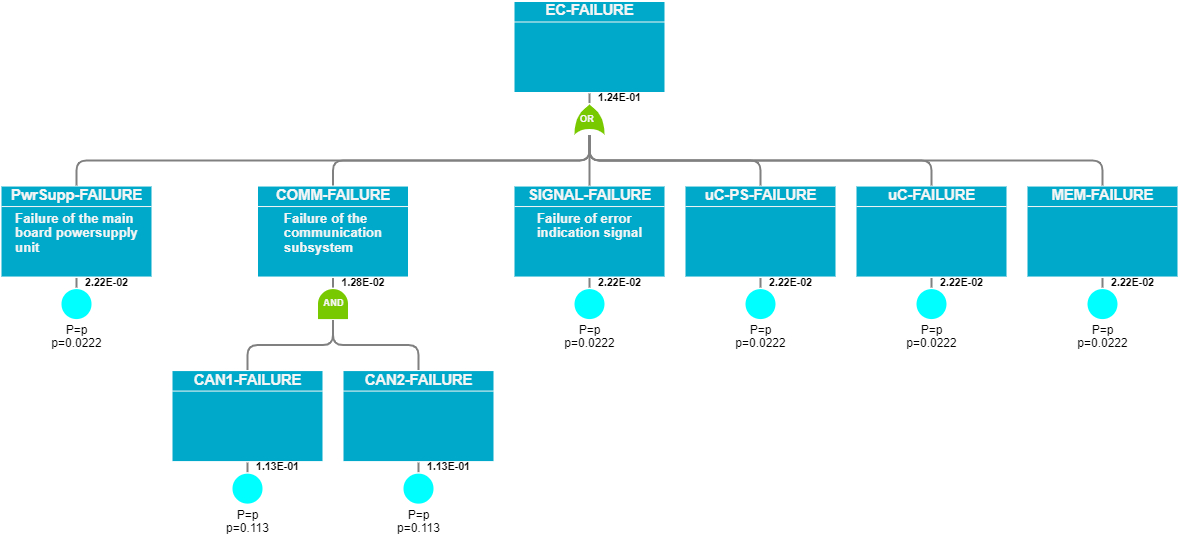
\includegraphics[width=150mm, keepaspectratio]{figures/QuantiFTA.png}
    \caption{Kvantitatív FTA az adott értékek alapján}
    \label{fig:quant}
\end{figure}

Amint az az \ref{fig:quant}. ábrán látható a kvantitatív analízis elvégzése után látható az alrendszer teljes élelttartamra számított detektálatlan hibájának a valószínűsége.
Ez sajnos nem egy szép alacsony szám, de vegyük figyelembe, hogy ez százötven-ezer órára vetített érték és még így is a rendszenszer számára allokált SIL kategóriába tartozik, sőt még a rendszer számára osztott TFFR-en is belül helyezkedik.
